\chapter{Nasazení}
\label{sec:dp}

\begin{figure}[h!]
    \centering
    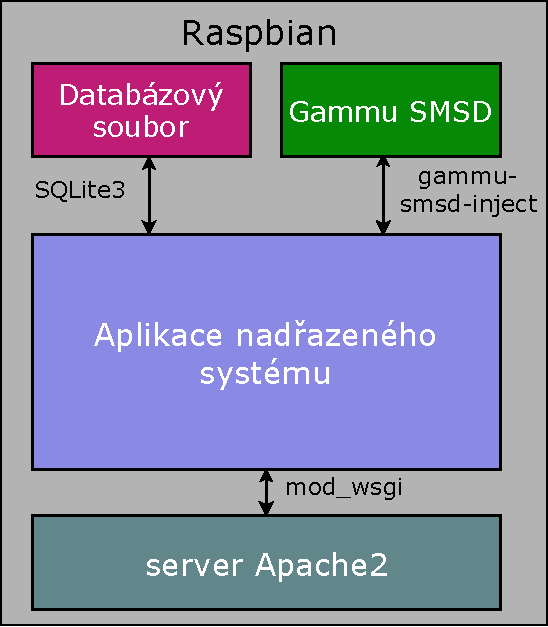
\includegraphics[width=0.8\textwidth]{images/sw_block.pdf}
    \caption[Softwarové blokové schéma nadřazeného systému]{Softwarové blokové schéma nadřazeného systému. Aplikace běží na OS Raspbian. Jako webový server je použit Apache2, se kterým aplikace komunikuje pomocí modulu mod\_wsgi \cite{mod_wsgi}. Databáze je upravována pomocí systému SQLite3, pro odesílání SMS s upozorněními je použit program Gammu (bližší informace v sekci \ref{sec:im_notifications}).}
    \label{fig:sw_block}
\end{figure}

V této kapitole je stručně popsáno nasazení aplikace nadřazeného systému na jednodeskovém počítači Raspberry Pi 3 s operačním systémem Raspbian. Blokové schéma nasazené aplikace je na obrázku \ref{fig:sw_block}. 

K instalaci a spuštění aplikace je zapotřebí tento software:

\begin{itemize}
    \item Webový server Apache2.
    \item Programovací jazyk Python3.
    \begin{itemize}
        \item Systém pro správu balíčků pip. %citace k pip
        % pomoci nej se nainstalujou pythnovsky zavislosti jako flask atd
    \end{itemize}
    \item Program pro ovádání GSM modulu Gammu. % optional, jen kdyz chceme smsky
\end{itemize}

\section{Konfigurace Apache2}

\subsection{Použité moduly}

\subsection{\textit{Self-signed} certifkikát}

\section{Konfigurace Gammu SMSD}

\section{Konfigurace RTC}